\section{Rectangle Class Reference}
\label{classRectangle}\index{Rectangle@{Rectangle}}
{\tt \#include $<$world.hpp$>$}

Collaboration diagram for Rectangle:\begin{figure}[H]
\begin{center}
\leavevmode
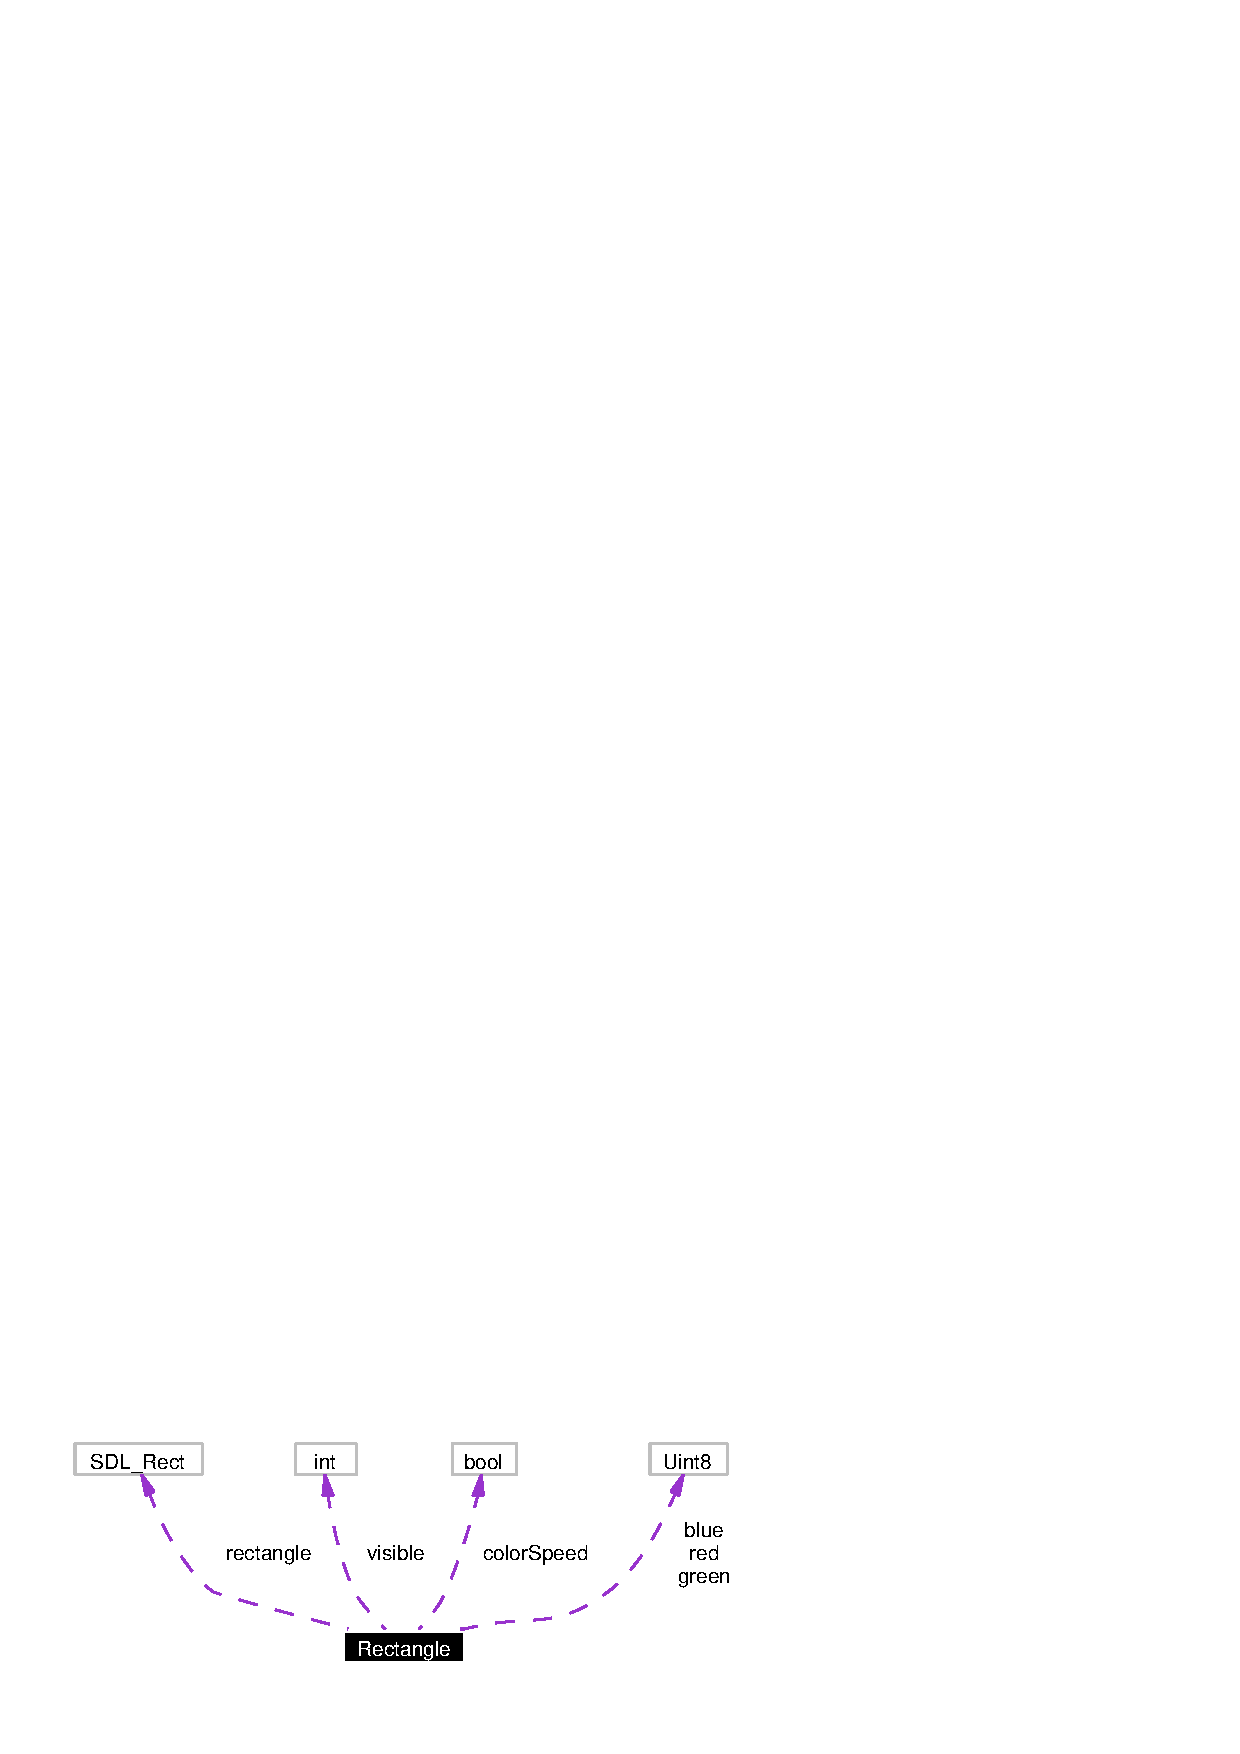
\includegraphics[width=184pt]{classRectangle__coll__graph}
\end{center}
\end{figure}
\subsection*{Public Member Functions}
\begin{CompactItemize}
\item 
void {\bf set\-Position} (Sint16 new\-Pos\-X, Sint16 new\-Pos\-Y)
\item 
Sint16 {\bf get\-Position\-X} (void)
\item 
Sint16 {\bf get\-Position\-Y} (void)
\item 
void {\bf set\-Size} (Uint16 new\-Width, Uint16 new\-Height)
\item 
Sint16 {\bf get\-Size\-X} (void)
\item 
Sint16 {\bf get\-Size\-Y} (void)
\item 
void {\bf set\-Visible} (int visibility)
\item 
int {\bf is\-Visible} ()
\item 
SDL\_\-Rect $\ast$ {\bf sdl\-Rectangle} ()
\end{CompactItemize}
\subsection*{Public Attributes}
\begin{CompactItemize}
\item 
Uint8 {\bf red}
\item 
Uint8 {\bf green}
\item 
Uint8 {\bf blue}
\item 
bool {\bf color\-Speed}
\end{CompactItemize}
\subsection*{Private Attributes}
\begin{CompactItemize}
\item 
SDL\_\-Rect {\bf rectangle}
\item 
int {\bf visible}
\end{CompactItemize}


\subsection{Member Function Documentation}
\index{Rectangle@{Rectangle}!getPositionX@{getPositionX}}
\index{getPositionX@{getPositionX}!Rectangle@{Rectangle}}
\subsubsection{\setlength{\rightskip}{0pt plus 5cm}Sint16 Rectangle::get\-Position\-X (void)}\label{classRectangle_a1}


\index{Rectangle@{Rectangle}!getPositionY@{getPositionY}}
\index{getPositionY@{getPositionY}!Rectangle@{Rectangle}}
\subsubsection{\setlength{\rightskip}{0pt plus 5cm}Sint16 Rectangle::get\-Position\-Y (void)}\label{classRectangle_a2}


\index{Rectangle@{Rectangle}!getSizeX@{getSizeX}}
\index{getSizeX@{getSizeX}!Rectangle@{Rectangle}}
\subsubsection{\setlength{\rightskip}{0pt plus 5cm}Sint16 Rectangle::get\-Size\-X (void)}\label{classRectangle_a4}


\index{Rectangle@{Rectangle}!getSizeY@{getSizeY}}
\index{getSizeY@{getSizeY}!Rectangle@{Rectangle}}
\subsubsection{\setlength{\rightskip}{0pt plus 5cm}Sint16 Rectangle::get\-Size\-Y (void)}\label{classRectangle_a5}


\index{Rectangle@{Rectangle}!isVisible@{isVisible}}
\index{isVisible@{isVisible}!Rectangle@{Rectangle}}
\subsubsection{\setlength{\rightskip}{0pt plus 5cm}int Rectangle::is\-Visible ()}\label{classRectangle_a7}


\index{Rectangle@{Rectangle}!sdlRectangle@{sdlRectangle}}
\index{sdlRectangle@{sdlRectangle}!Rectangle@{Rectangle}}
\subsubsection{\setlength{\rightskip}{0pt plus 5cm}SDL\_\-Rect $\ast$ Rectangle::sdl\-Rectangle ()}\label{classRectangle_a8}


\index{Rectangle@{Rectangle}!setPosition@{setPosition}}
\index{setPosition@{setPosition}!Rectangle@{Rectangle}}
\subsubsection{\setlength{\rightskip}{0pt plus 5cm}void Rectangle::set\-Position (Sint16 {\em new\-Pos\-X}, Sint16 {\em new\-Pos\-Y})}\label{classRectangle_a0}


\index{Rectangle@{Rectangle}!setSize@{setSize}}
\index{setSize@{setSize}!Rectangle@{Rectangle}}
\subsubsection{\setlength{\rightskip}{0pt plus 5cm}void Rectangle::set\-Size (Uint16 {\em new\-Width}, Uint16 {\em new\-Height})}\label{classRectangle_a3}


\index{Rectangle@{Rectangle}!setVisible@{setVisible}}
\index{setVisible@{setVisible}!Rectangle@{Rectangle}}
\subsubsection{\setlength{\rightskip}{0pt plus 5cm}void Rectangle::set\-Visible (int {\em visibility})}\label{classRectangle_a6}




\subsection{Member Data Documentation}
\index{Rectangle@{Rectangle}!blue@{blue}}
\index{blue@{blue}!Rectangle@{Rectangle}}
\subsubsection{\setlength{\rightskip}{0pt plus 5cm}Uint8 {\bf Rectangle::blue}}\label{classRectangle_o2}


\index{Rectangle@{Rectangle}!colorSpeed@{colorSpeed}}
\index{colorSpeed@{colorSpeed}!Rectangle@{Rectangle}}
\subsubsection{\setlength{\rightskip}{0pt plus 5cm}bool {\bf Rectangle::color\-Speed}}\label{classRectangle_o3}


\index{Rectangle@{Rectangle}!green@{green}}
\index{green@{green}!Rectangle@{Rectangle}}
\subsubsection{\setlength{\rightskip}{0pt plus 5cm}Uint8 {\bf Rectangle::green}}\label{classRectangle_o1}


\index{Rectangle@{Rectangle}!rectangle@{rectangle}}
\index{rectangle@{rectangle}!Rectangle@{Rectangle}}
\subsubsection{\setlength{\rightskip}{0pt plus 5cm}SDL\_\-Rect {\bf Rectangle::rectangle}\hspace{0.3cm}{\tt  [private]}}\label{classRectangle_r0}


\index{Rectangle@{Rectangle}!red@{red}}
\index{red@{red}!Rectangle@{Rectangle}}
\subsubsection{\setlength{\rightskip}{0pt plus 5cm}Uint8 {\bf Rectangle::red}}\label{classRectangle_o0}


\index{Rectangle@{Rectangle}!visible@{visible}}
\index{visible@{visible}!Rectangle@{Rectangle}}
\subsubsection{\setlength{\rightskip}{0pt plus 5cm}int {\bf Rectangle::visible}\hspace{0.3cm}{\tt  [private]}}\label{classRectangle_r1}




The documentation for this class was generated from the following files:\begin{CompactItemize}
\item 
src/{\bf world.hpp}\item 
src/{\bf world.cpp}\end{CompactItemize}
